% ---------------------------------------------------------------------------
% Homework 1 report --- Introduction to Artificial Intelligence (2026 Fall)
%
% Base template: Overleaf "COSC-4765-HW2-TEMPLATE" (single-file assignment
% template, article + fancyhdr).  Source page:
%   https://www.overleaf.com/latex/templates/cosc-4765-hw2-template/ghhnykqjbdgd
%
% Submit as: report_<student_id>.pdf
% ---------------------------------------------------------------------------
\documentclass[11pt]{article}
\usepackage[utf8]{inputenc}
\usepackage[T1]{fontenc}
\usepackage[margin=1in]{geometry}
\usepackage{enumitem}
\usepackage{fancyhdr}
\usepackage{amsmath,amssymb}
\usepackage{graphicx}
\usepackage{booktabs}
\usepackage{needspace}
\pagestyle{fancy}
\setlength{\headheight}{14pt}

\title{Homework 1}
\author{Lixi Zhang\\ Student ID: 2025011067}
\lhead{Lixi Zhang}
\rhead{2025011067}

\begin{document}
\maketitle

% ===========================================================================
\section*{Q1}

\subsection*{Q1.1 Search with Heuristics}

\subsubsection*{(a) Size of the state space}
A state assigns the $n$ labelled cars to $n$ distinct cells of the $n\times n$
grid, so the exact number of states is
\[
    \binom{n^{2}}{n} n! = n^{2}(n^{2}-1)\cdots(n^{2}-n+1) = \Theta(n^{2n}),
\]
i.e.\ $O(n^{2n})$.

\subsubsection*{(b) Admissibility of $h_i$}
With a single car the grid is empty, so the shortest path to the goal is exactly
the Manhattan distance and $h_i$ is admissible. With the other
$n-1$ cars on the grid it is \emph{not} admissible: a stationary car can be
hopped over, covering two cells at cost $1$, so the true cost can be smaller
than $h_i$.
\subsubsection*{(c) Admissible candidates}

\begin{center}
\begin{tabular}{lll}
    \toprule
    candidate & admissible & reason \\
    \midrule
    (i) $\sum_i h_i$     & no & $n=3$, cars $(1,1),(1,2),(1,3)$: $\sum_i h_i = 6$, true cost $5$ \\
    (ii) $\min_i h_i$    & \textbf{yes} & each car needs $\lceil h_j/2\rceil$ moves, hence
                                            $h^{*}\ge n\lceil \min_i h_i/2\rceil \ge \min_i h_i$ \\
    (iii) $\max_i h_i$   & no & $n=3$, cars $(1,1),(2,3),(1,2)$: $\max_i h_i = 4$, true cost $3$ \\
    (iv) $n\min_i h_i$   & no & $n=3$, cars $(1,1),(2,1),(2,2)$: $n\min_i h_i = 6$, true cost $5$ \\
    (v) $n\max_i h_i$    & no & $n=3$, cars $(1,1),(2,1),(2,2)$: $n\max_i h_i = 12$, true cost $5$ \\
    \bottomrule
\end{tabular}
\end{center}

\subsection*{Q1.2 Adjusted Heuristics}

\begin{center}
    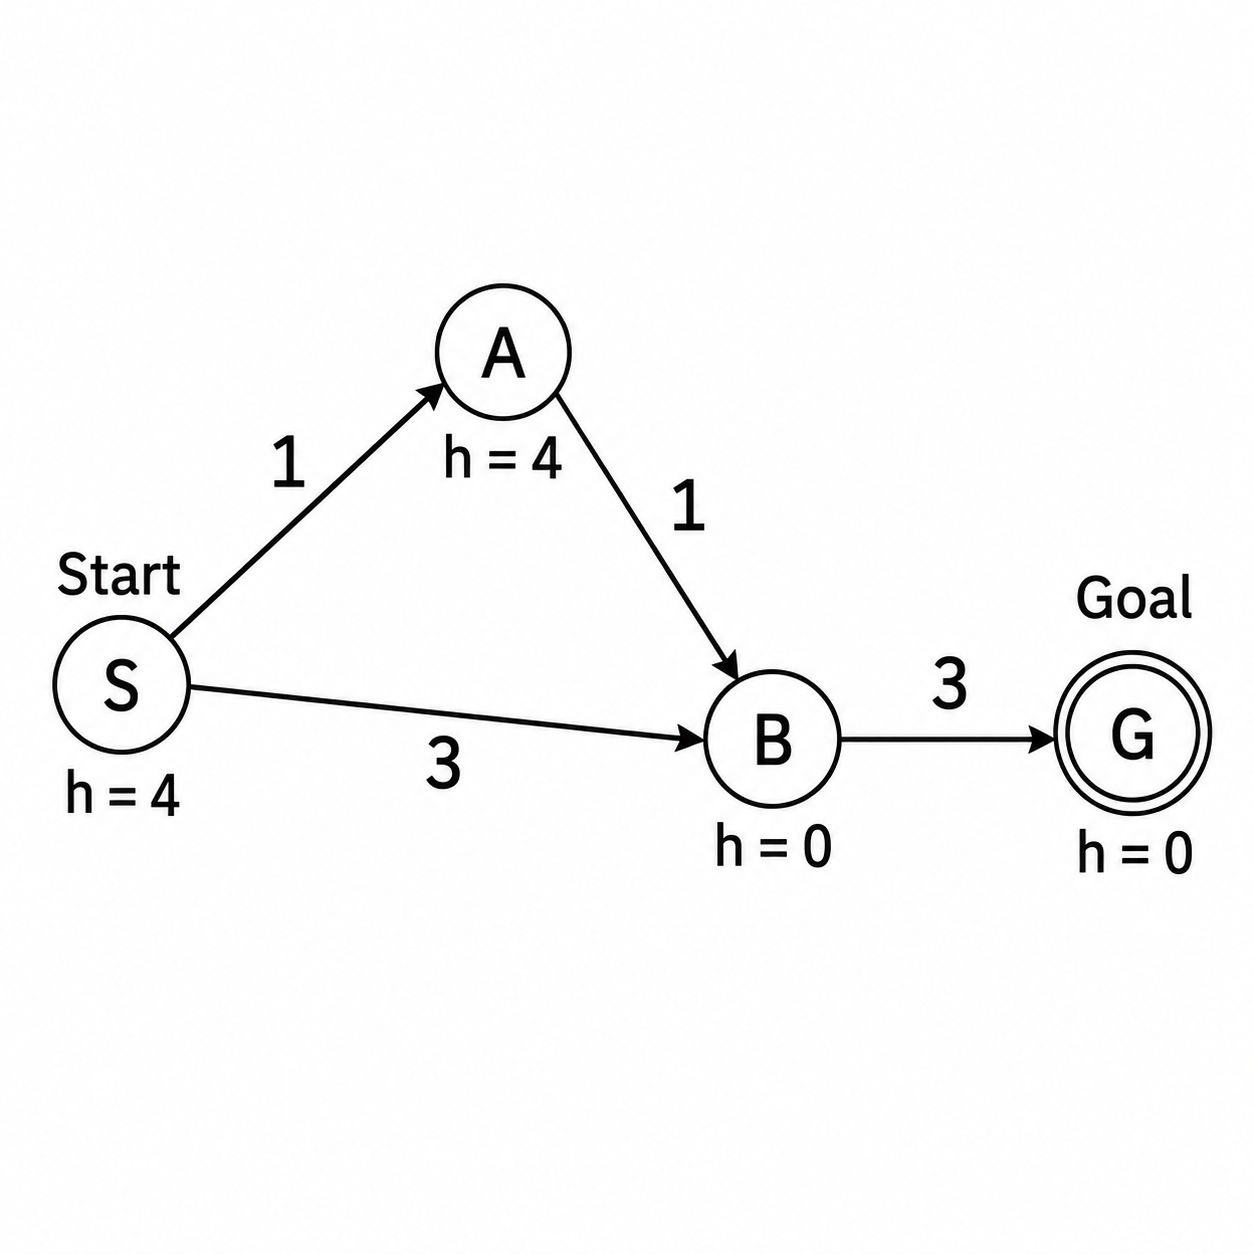
\includegraphics[width=0.55\linewidth]{1.2.png}
\end{center}

Take the graph above with $h(S)=4$, $h(A)=4$, $h(B)=0$, $h(G)=0$: admissible
($h^{*}=5,4,3,0$) but inconsistent on $S\to B$. Expanding $S$ raises
$h(B)=\max(0,4-3)=1$, so $B$ is filled in first by the long path $S\to B$ with
$g=3$ and is expanded before $A$, i.e.\ with $g=3$ instead of $g^{*}(B)=2$. When
$A$ is expanded afterwards, the shorter path $A\to B$ with $g=2$ can no longer be
extended to $B$, since $B$ is already closed.

\subsection*{Q1.3 Adversarial Search}

\subsubsection*{(a) Game tree}

\begin{center}
    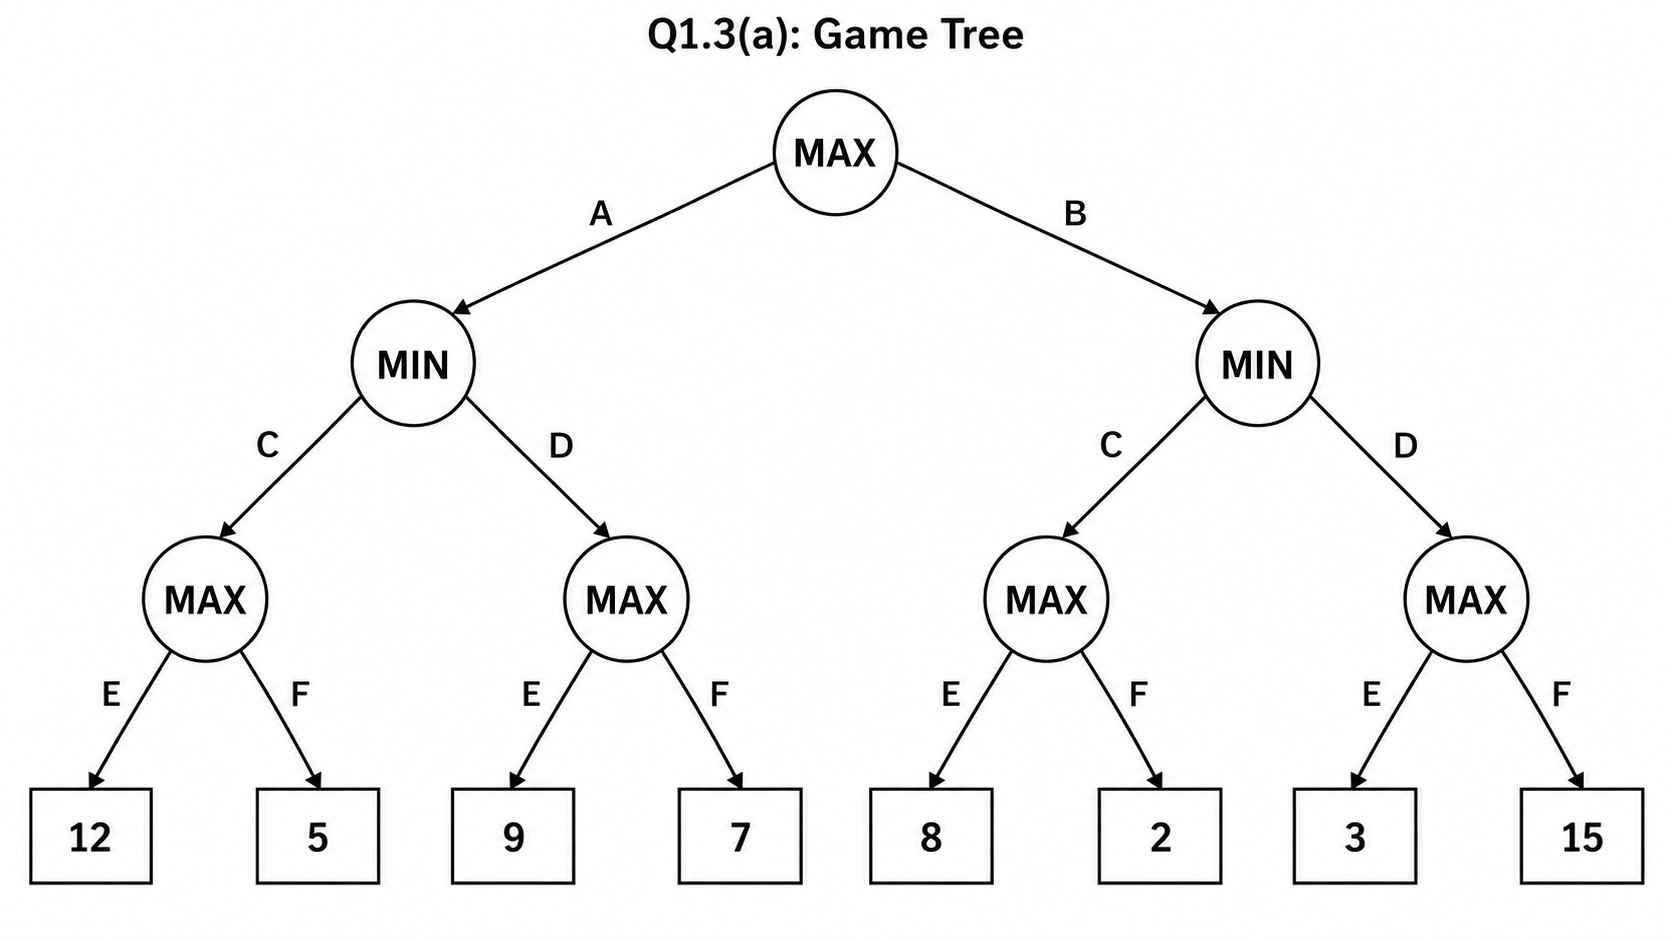
\includegraphics[width=0.78\linewidth]{1.3a.png}
\end{center}

\subsubsection*{(b) Minimax value of the root}
The minimax value of the root is 9.

\begin{center}
    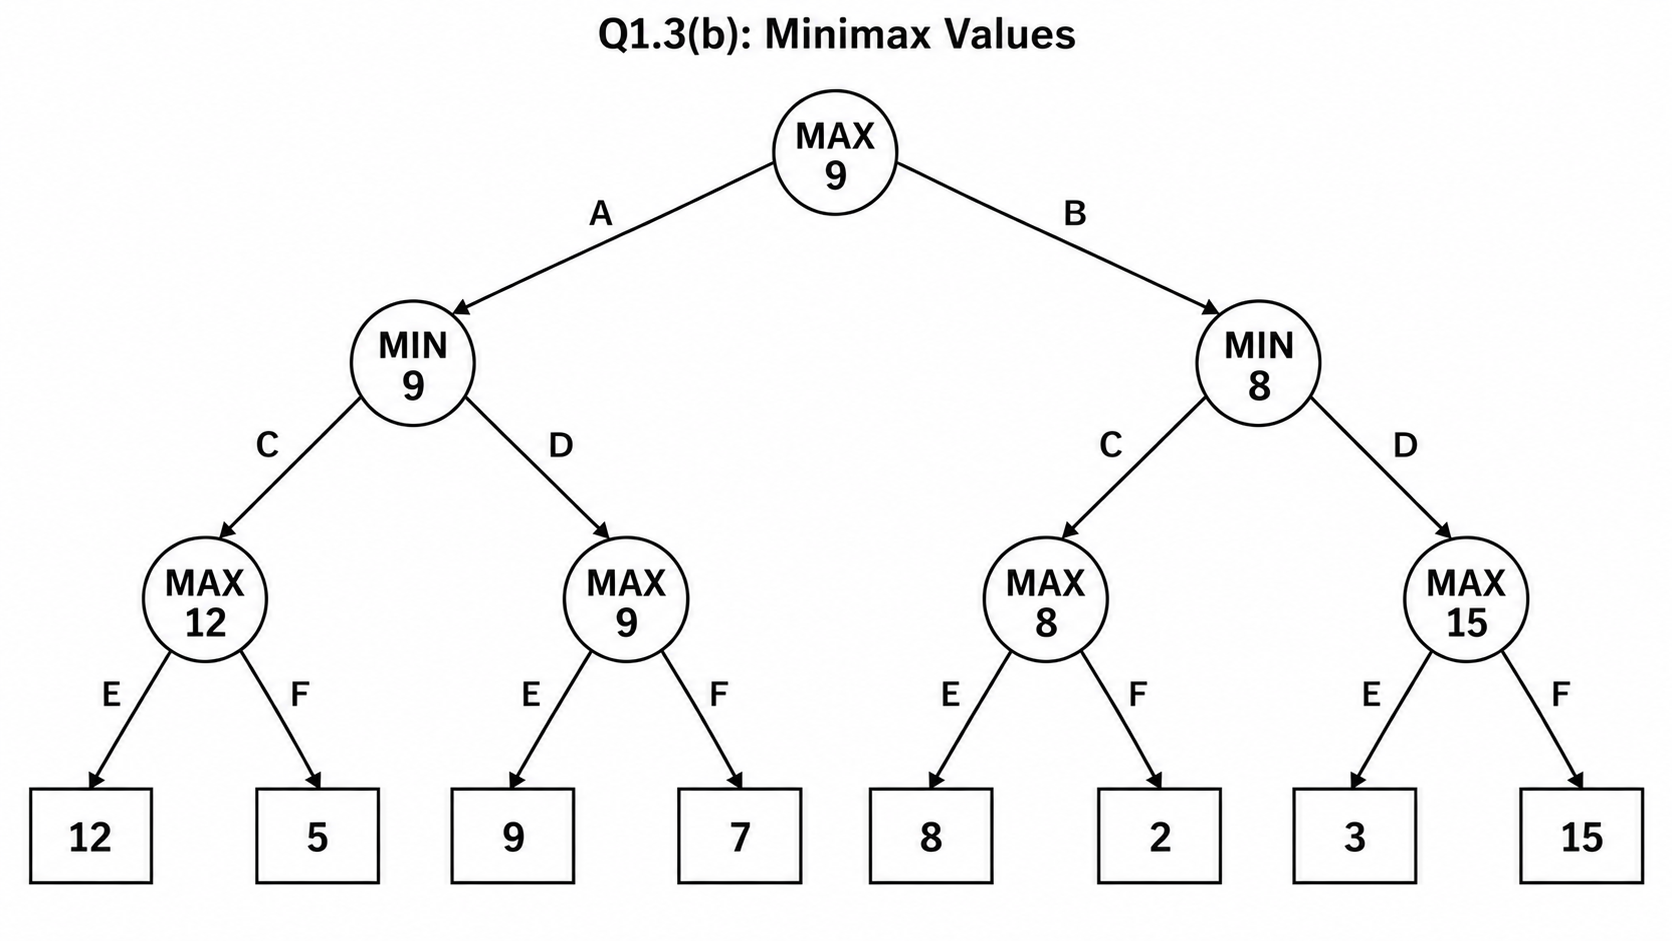
\includegraphics[width=0.78\linewidth]{1.3b.png}
\end{center}

\subsubsection*{(c) Alpha--beta pruning}
Traversing left to right, the last MAX node on the third level is pruned:
before it is entered, $\alpha = 9$, while its MIN parent already holds $8$.

% ===========================================================================
\needspace{0.68\textheight}
\section*{Q2}

\needspace{0.68\textheight}
\subsection*{Q2.1 Depth-first search}
Graph search with a \texttt{util.Stack}. On \texttt{mediumMaze} it reaches the
goal in 130 steps after expanding 146 nodes: the path is legal, but as expected
not optimal.

\begin{center}
    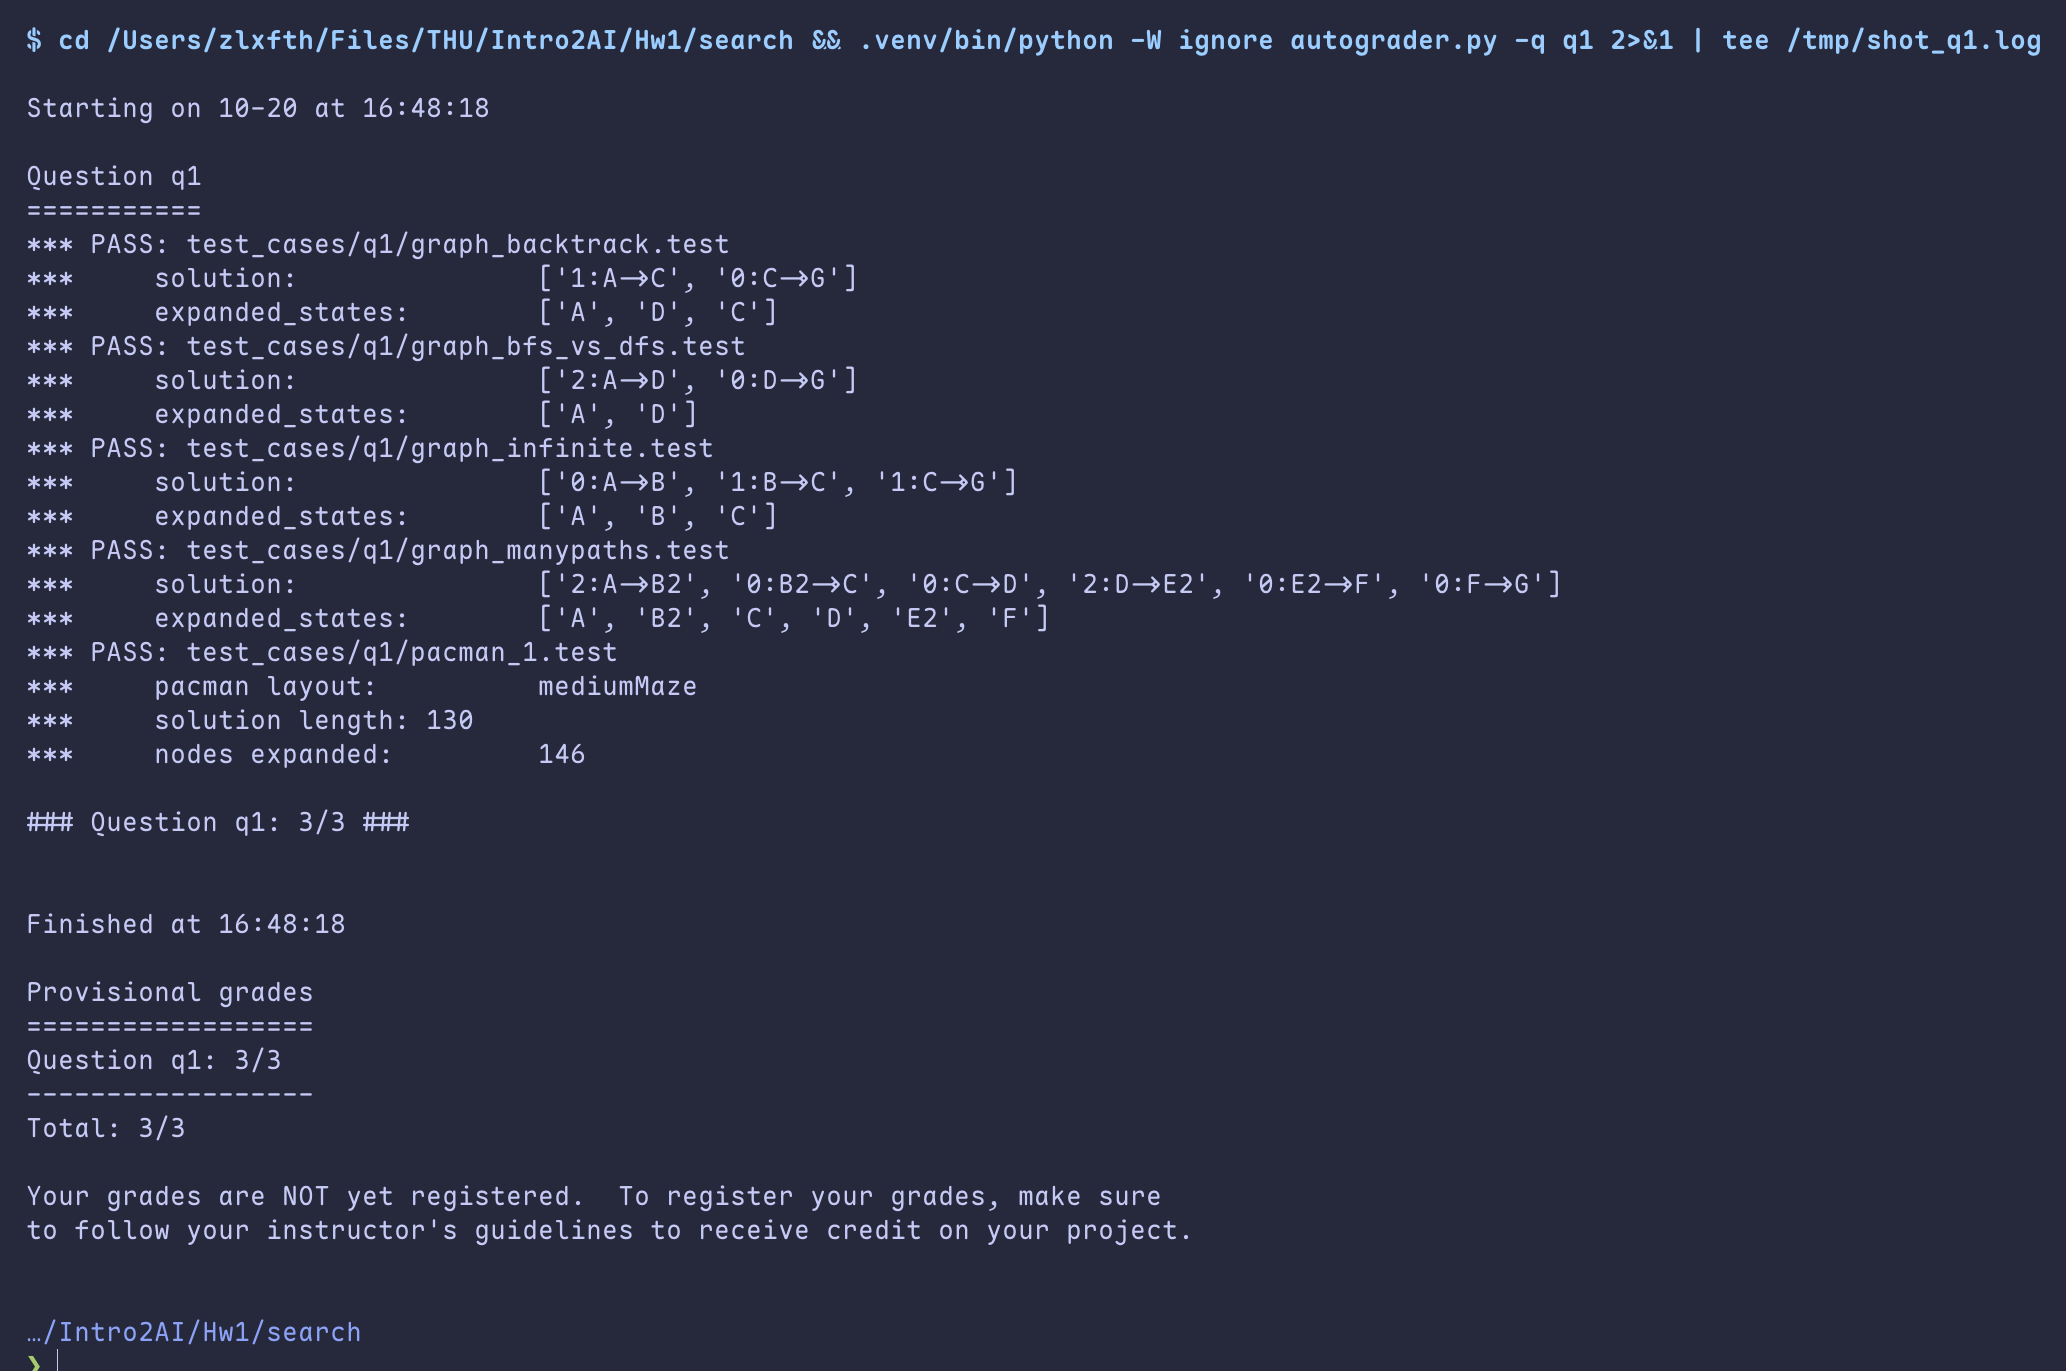
\includegraphics[width=0.85\linewidth]{../screenshot/q1.png}
\end{center}

\needspace{0.68\textheight}
\subsection*{Q2.2 Breadth-first search}
The same skeleton with a \texttt{util.Queue}. BFS does find a least-cost
solution: 68 steps on \texttt{mediumMaze}, against 130 for DFS, with 269 nodes
expanded.

\begin{center}
    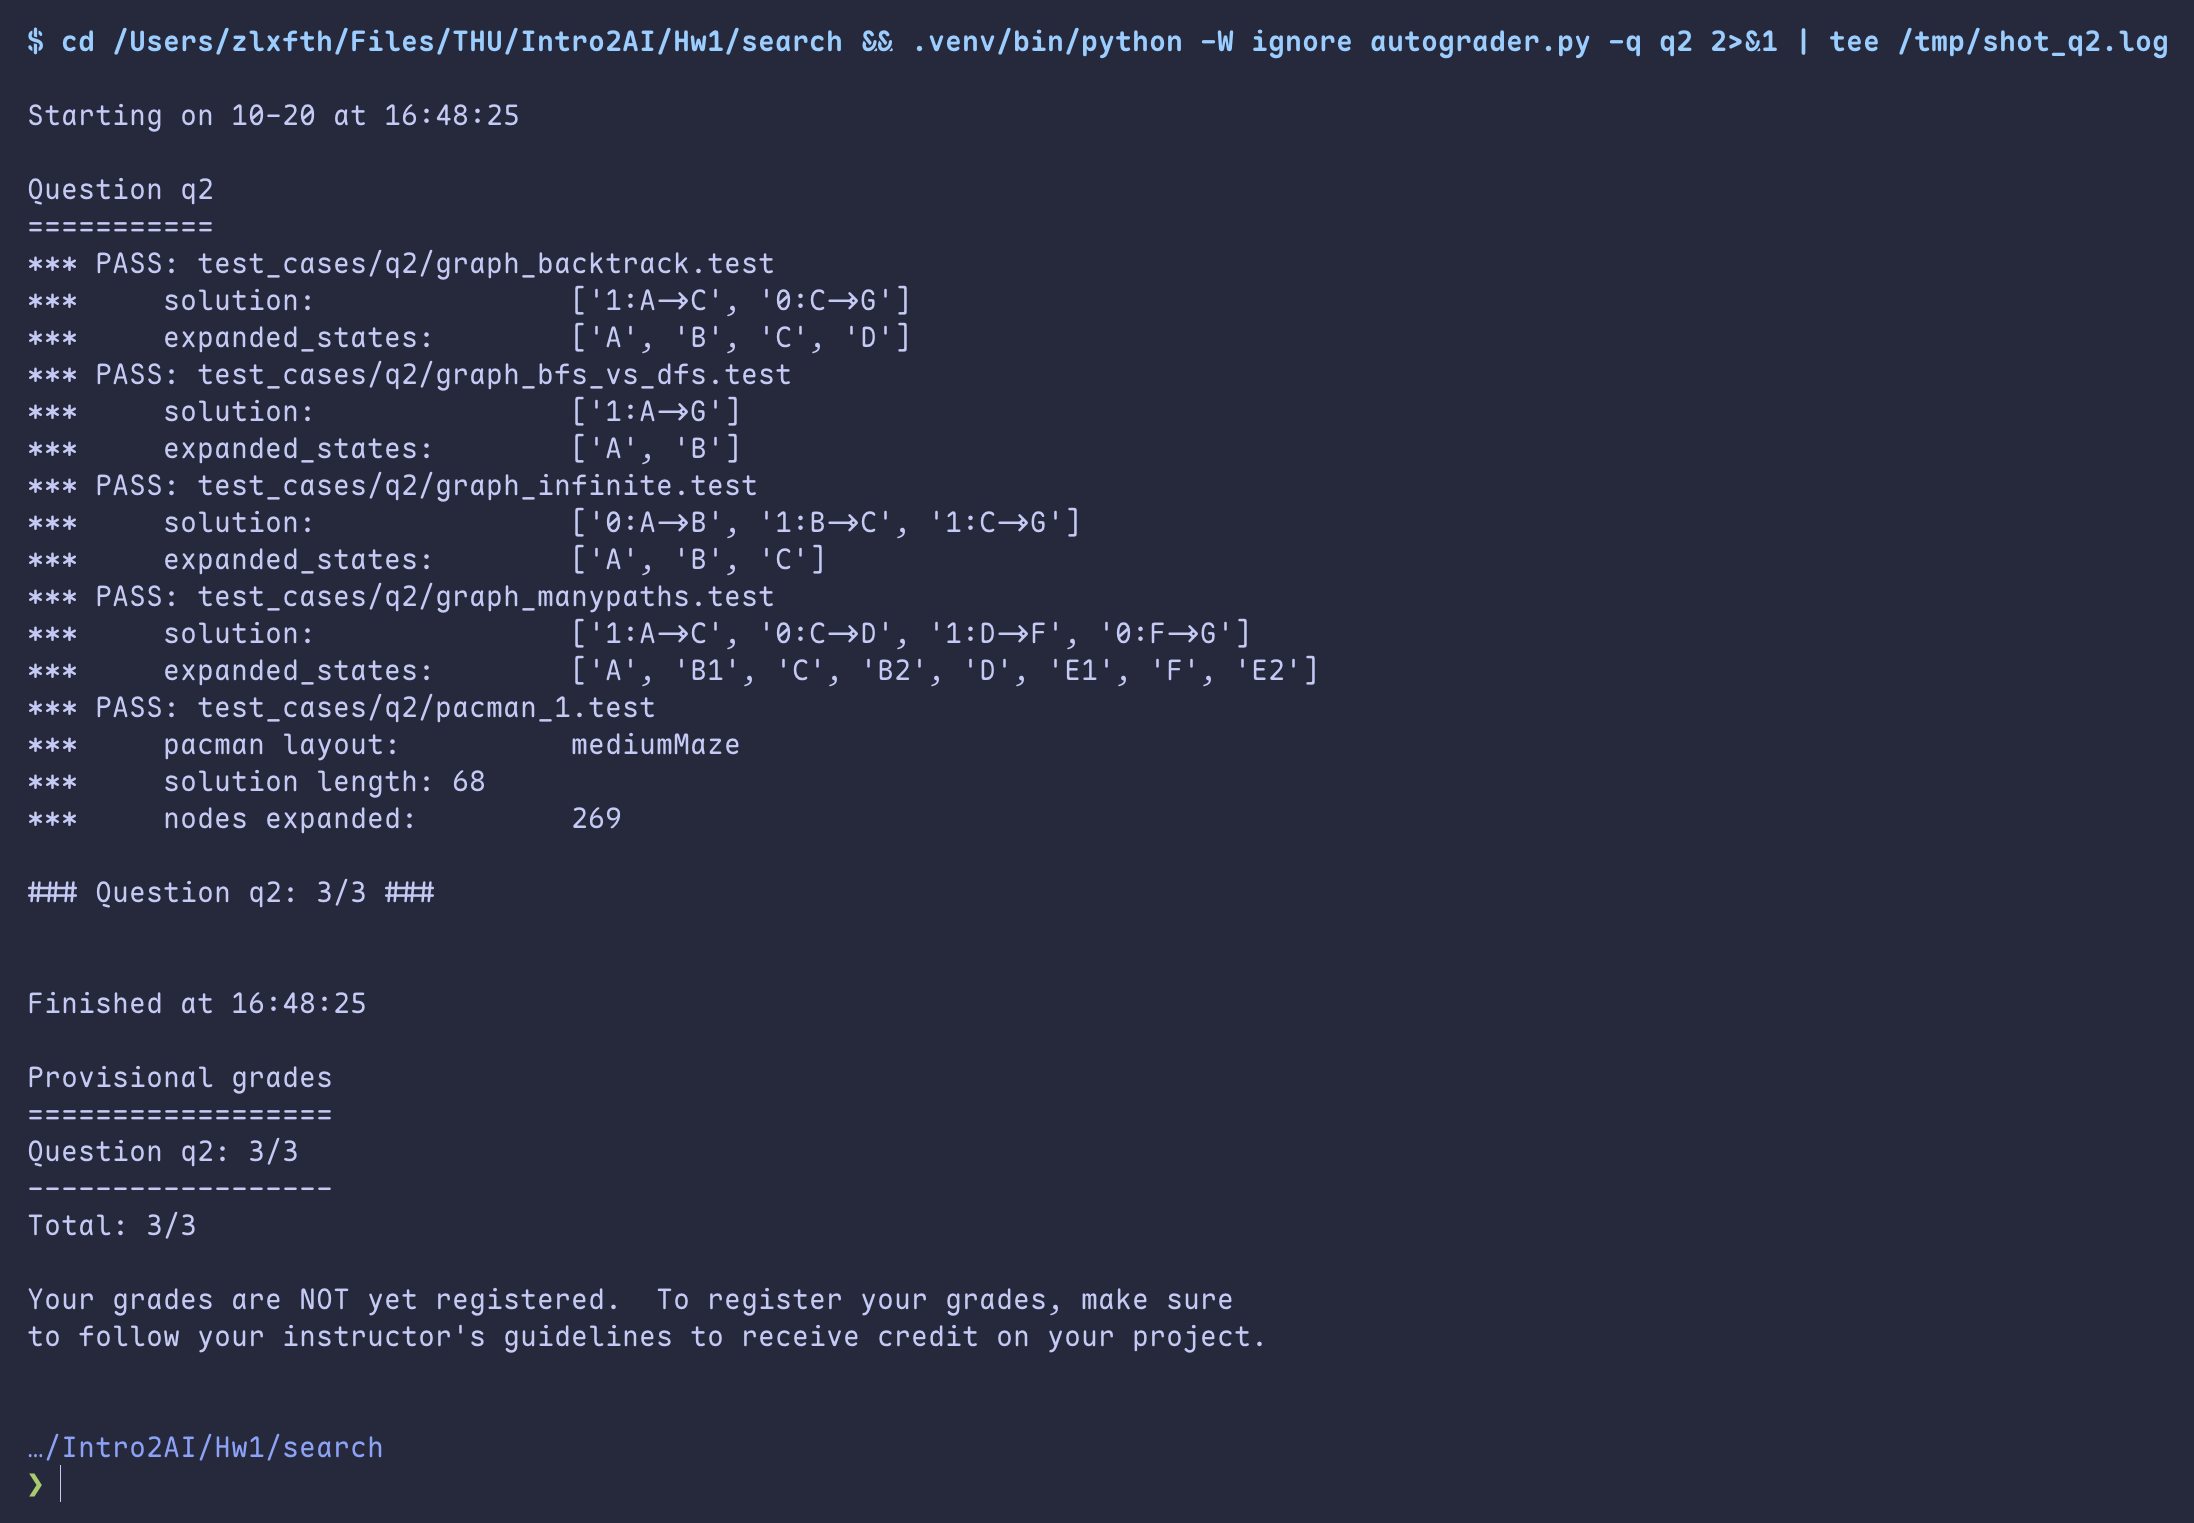
\includegraphics[width=0.85\linewidth]{../screenshot/q2.png}
\end{center}

\needspace{0.68\textheight}
\subsection*{Q2.3 Uniform-cost search}
The fringe is a priority queue keyed on $g$, and the goal test is applied on
dequeue (\texttt{ucs\_5\_goalAtDequeue}). With unit step costs UCS coincides
with BFS; with the exponential costs of \texttt{StayEastSearchAgent}
($0.5^{x}$, \texttt{mediumDottedMaze}) and \texttt{StayWestSearchAgent}
($2^{x}$, \texttt{mediumScaryMaze}) Pacman hugs the east and the west side
respectively, so the costs $68$, $1$ and $6.87\times10^{10}$ all come from the
\emph{same} algorithm under three different cost functions.

\begin{center}
    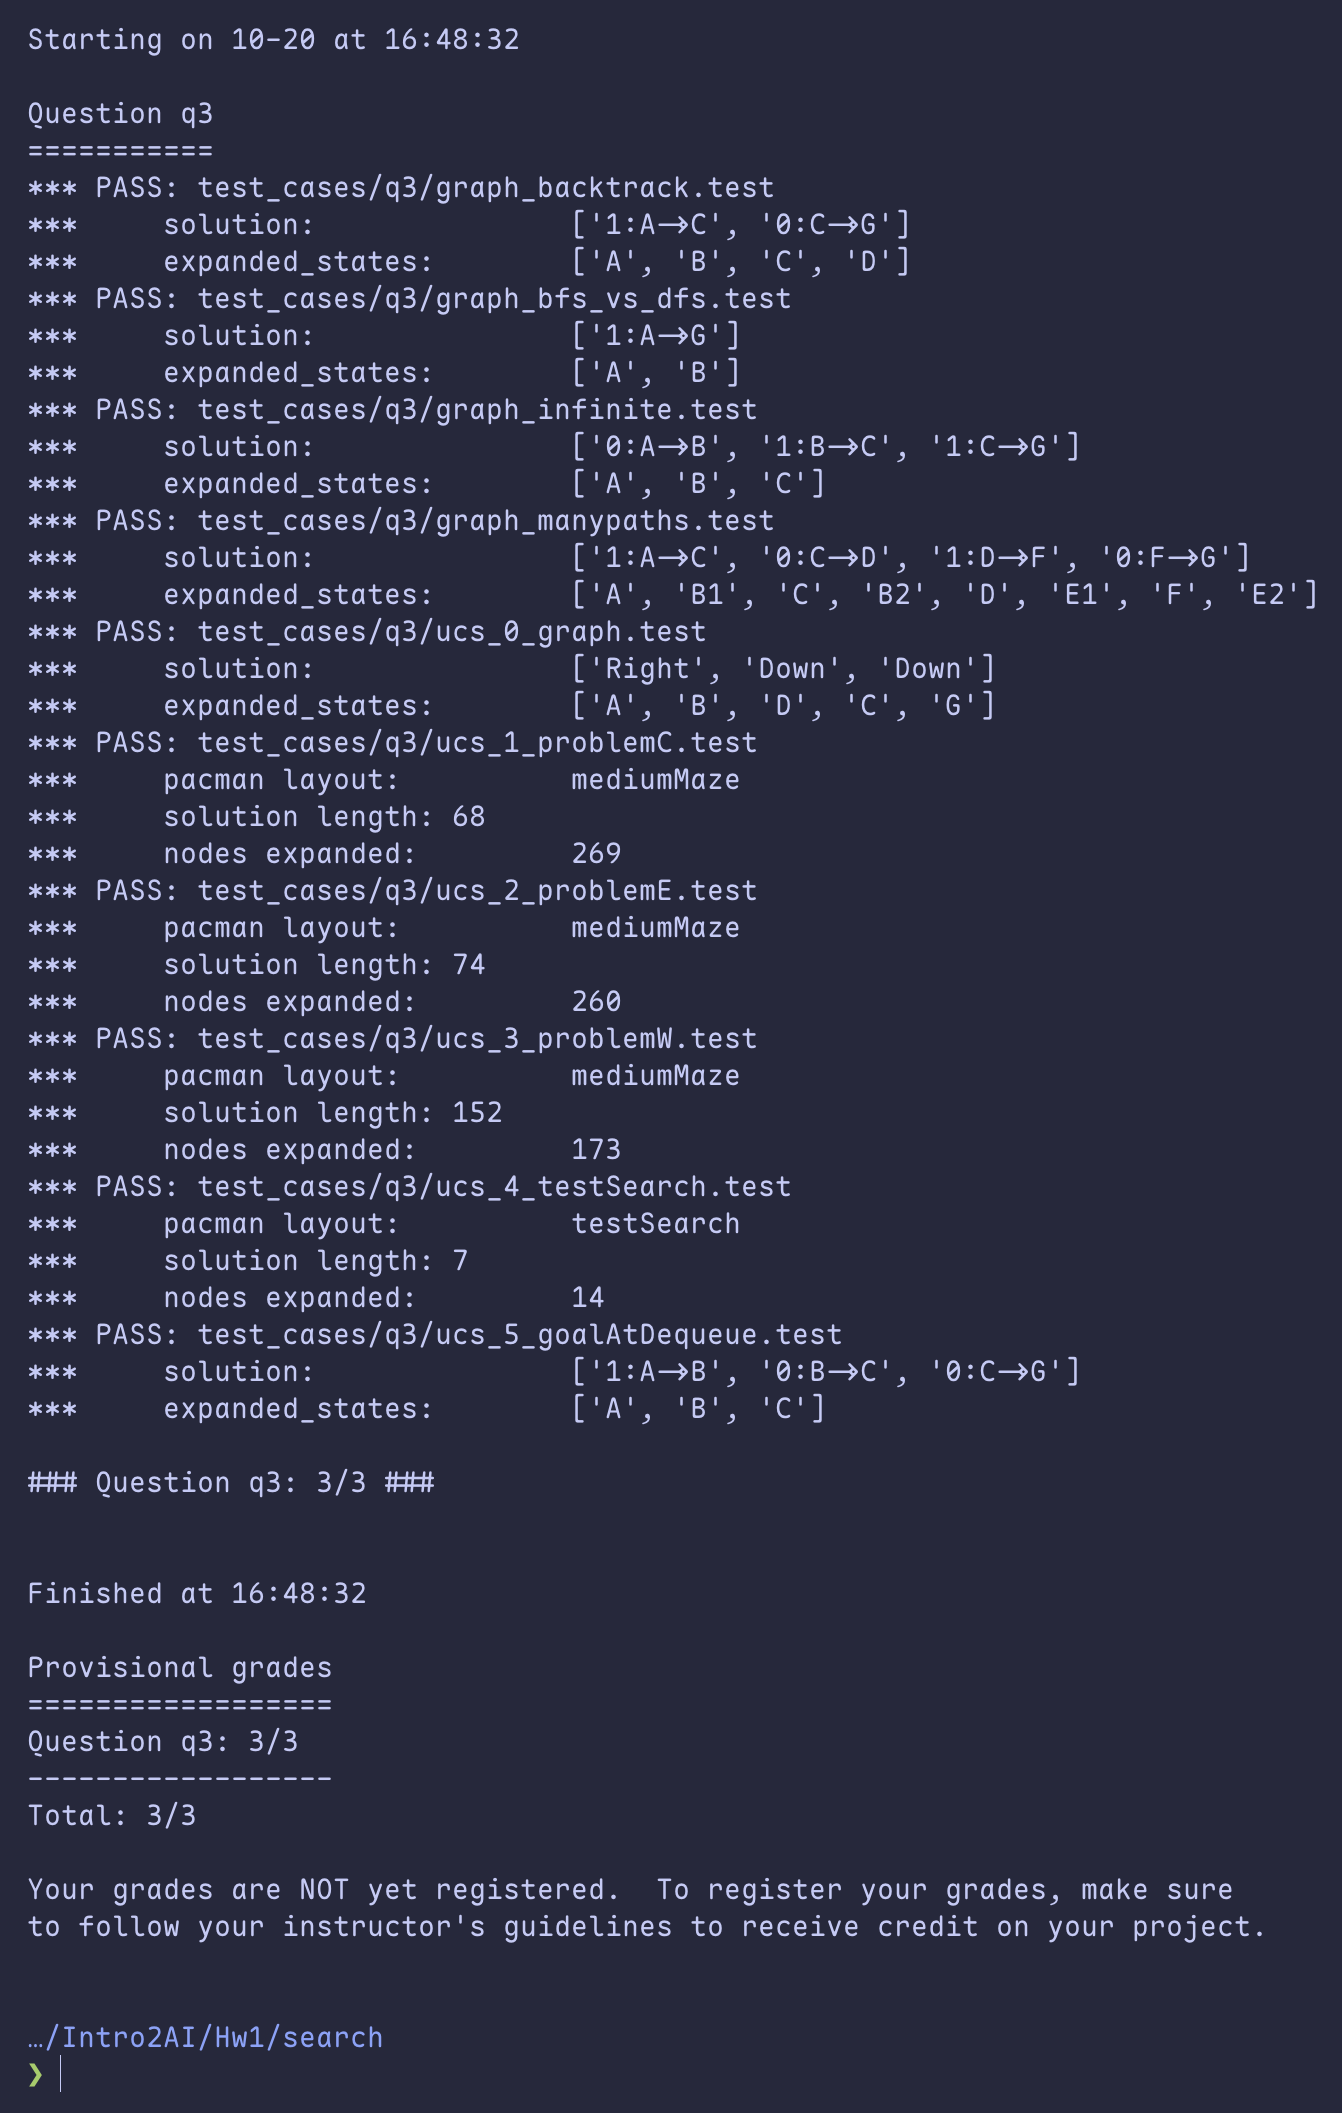
\includegraphics[height=0.48\textheight]{../screenshot/q3.png}
\end{center}

\needspace{0.68\textheight}
\subsection*{Q2.4 A$^*$ search}
The priority is $f = g + h$ with $h$ the Manhattan distance. On \texttt{bigMaze}
A$^*$ expands 549 nodes against 620 for UCS and returns the same optimal path of
cost 210. On the almost empty \texttt{openMaze} the differences are starker:

\begin{center}
\begin{tabular}{lrr}
    \toprule
    algorithm & nodes expanded & path cost \\
    \midrule
    DFS        & 576 & 298 \\
    BFS        & 682 & 54  \\
    UCS        & 682 & 54  \\
    A$^*$      & 535 & 54  \\
    \bottomrule
\end{tabular}
\end{center}

Without walls Manhattan is almost the exact remaining cost, so A$^*$ only
expands a narrow cone towards the goal, while BFS/UCS must sweep a whole
diamond; DFS simply gets lucky along one corridor and pays for it with a path
$5.5\times$ longer.

\begin{center}
    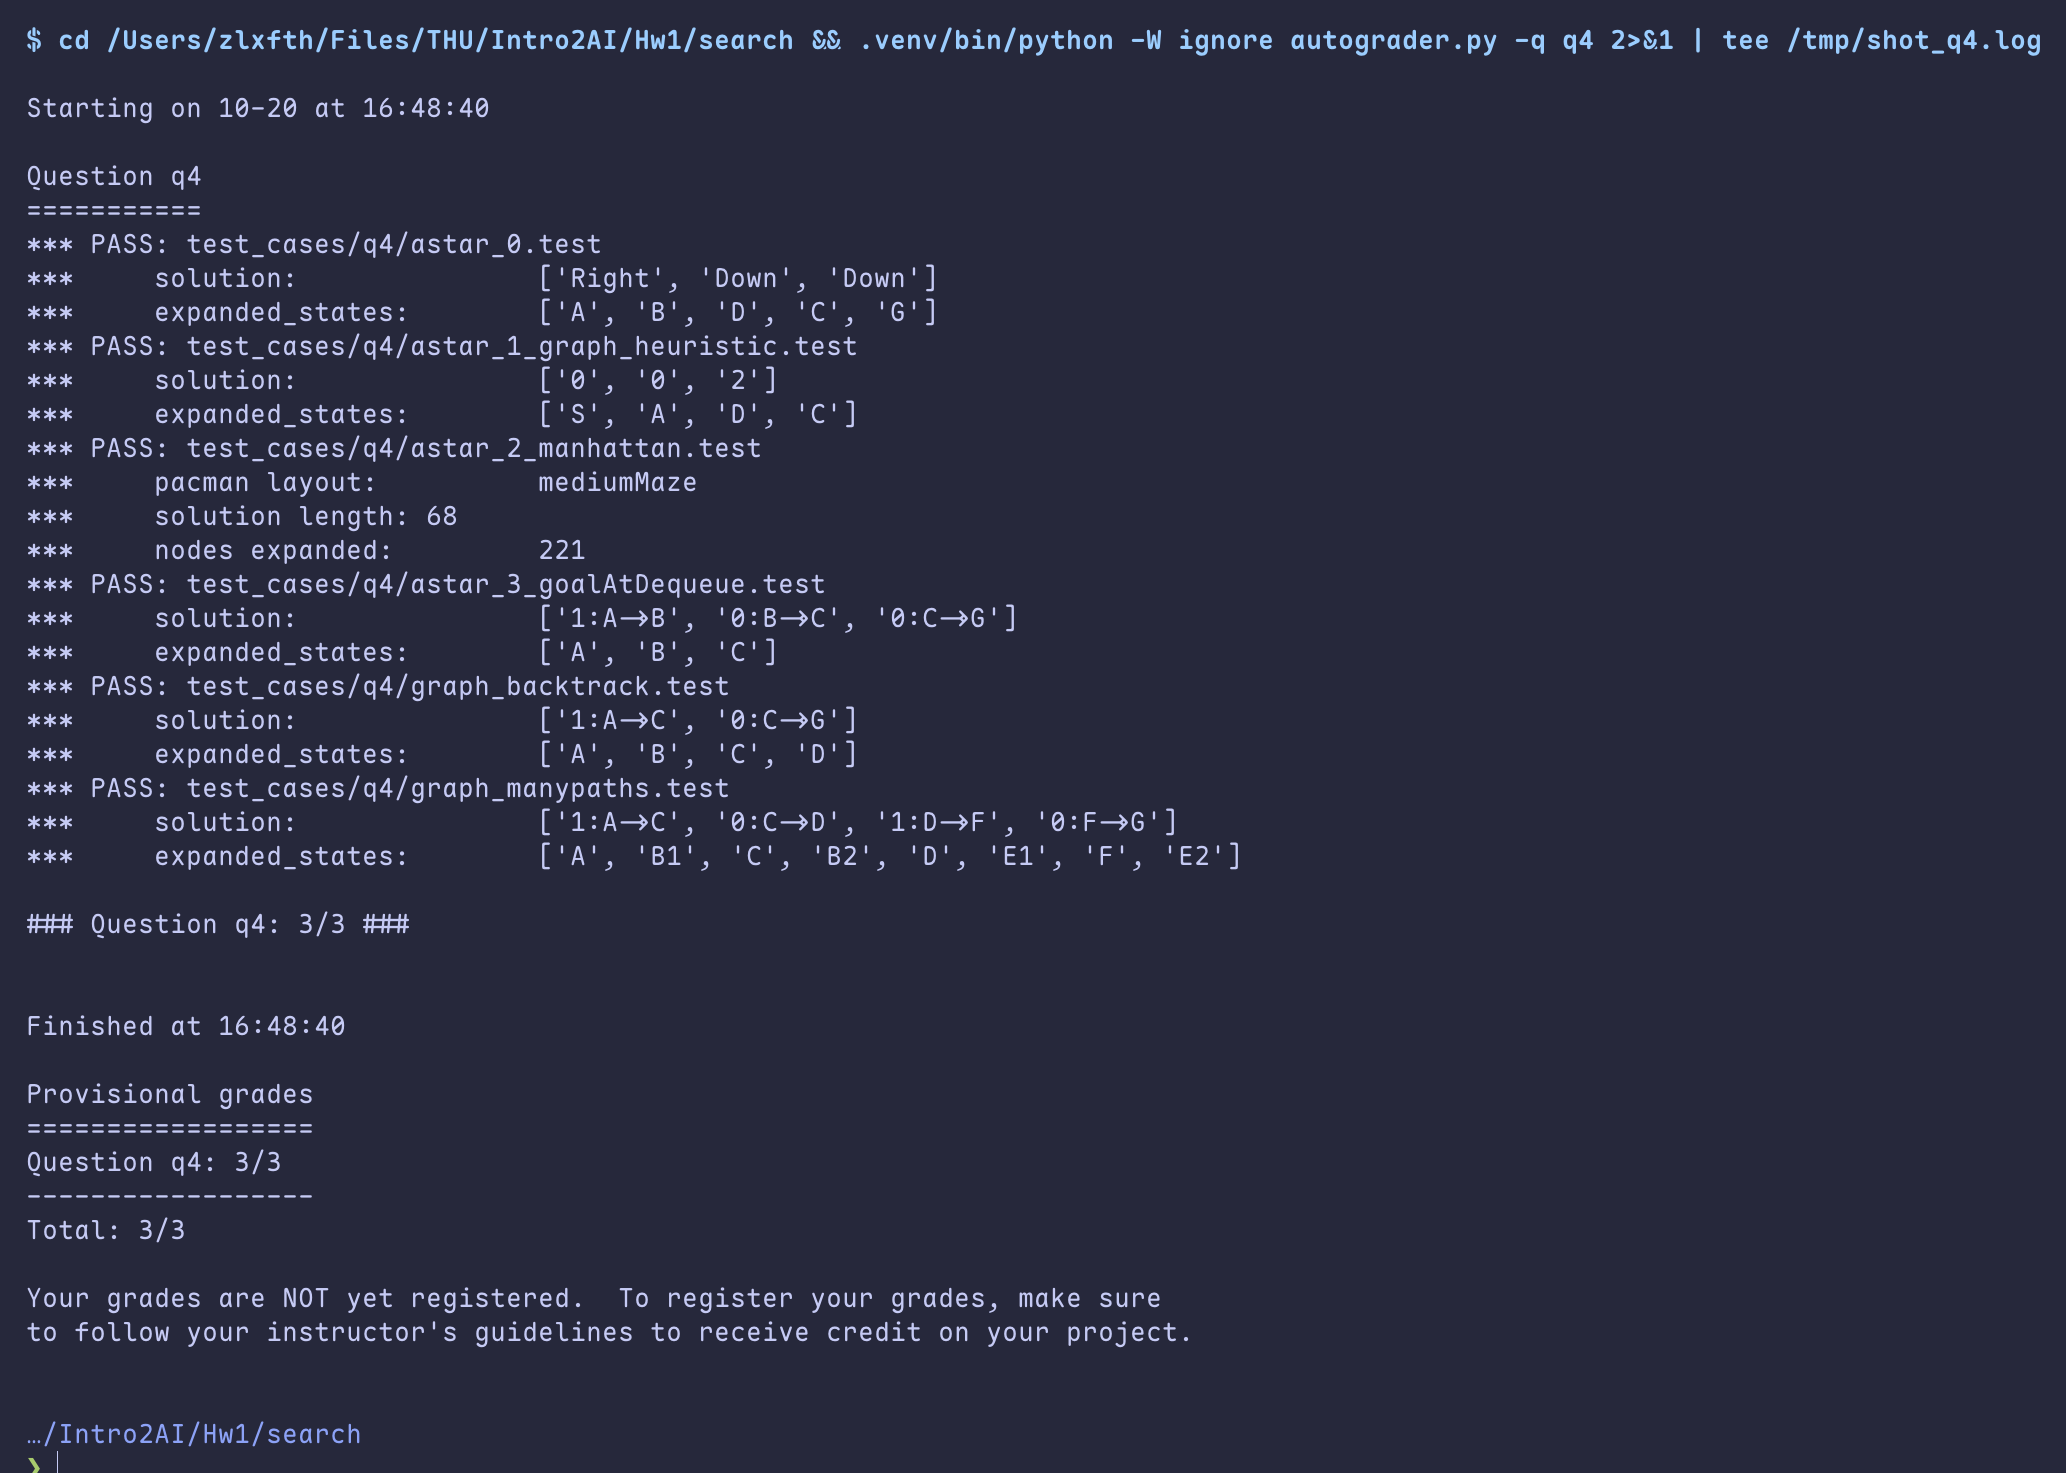
\includegraphics[width=0.85\linewidth]{../screenshot/q4.png}
\end{center}

\needspace{0.68\textheight}
\subsection*{Q2.5 Corners problem}
The state is $(\text{position},\ \text{frozenset of visited corners})$, the only
information the goal test needs; the start state is
$(\text{startingPosition},\ \varnothing)$. BFS then walks the four corners in
the optimal 28 steps on \texttt{tinyCorners} and expands 1966 nodes on
\texttt{mediumCorners} (``just under 2000'').

\begin{center}
    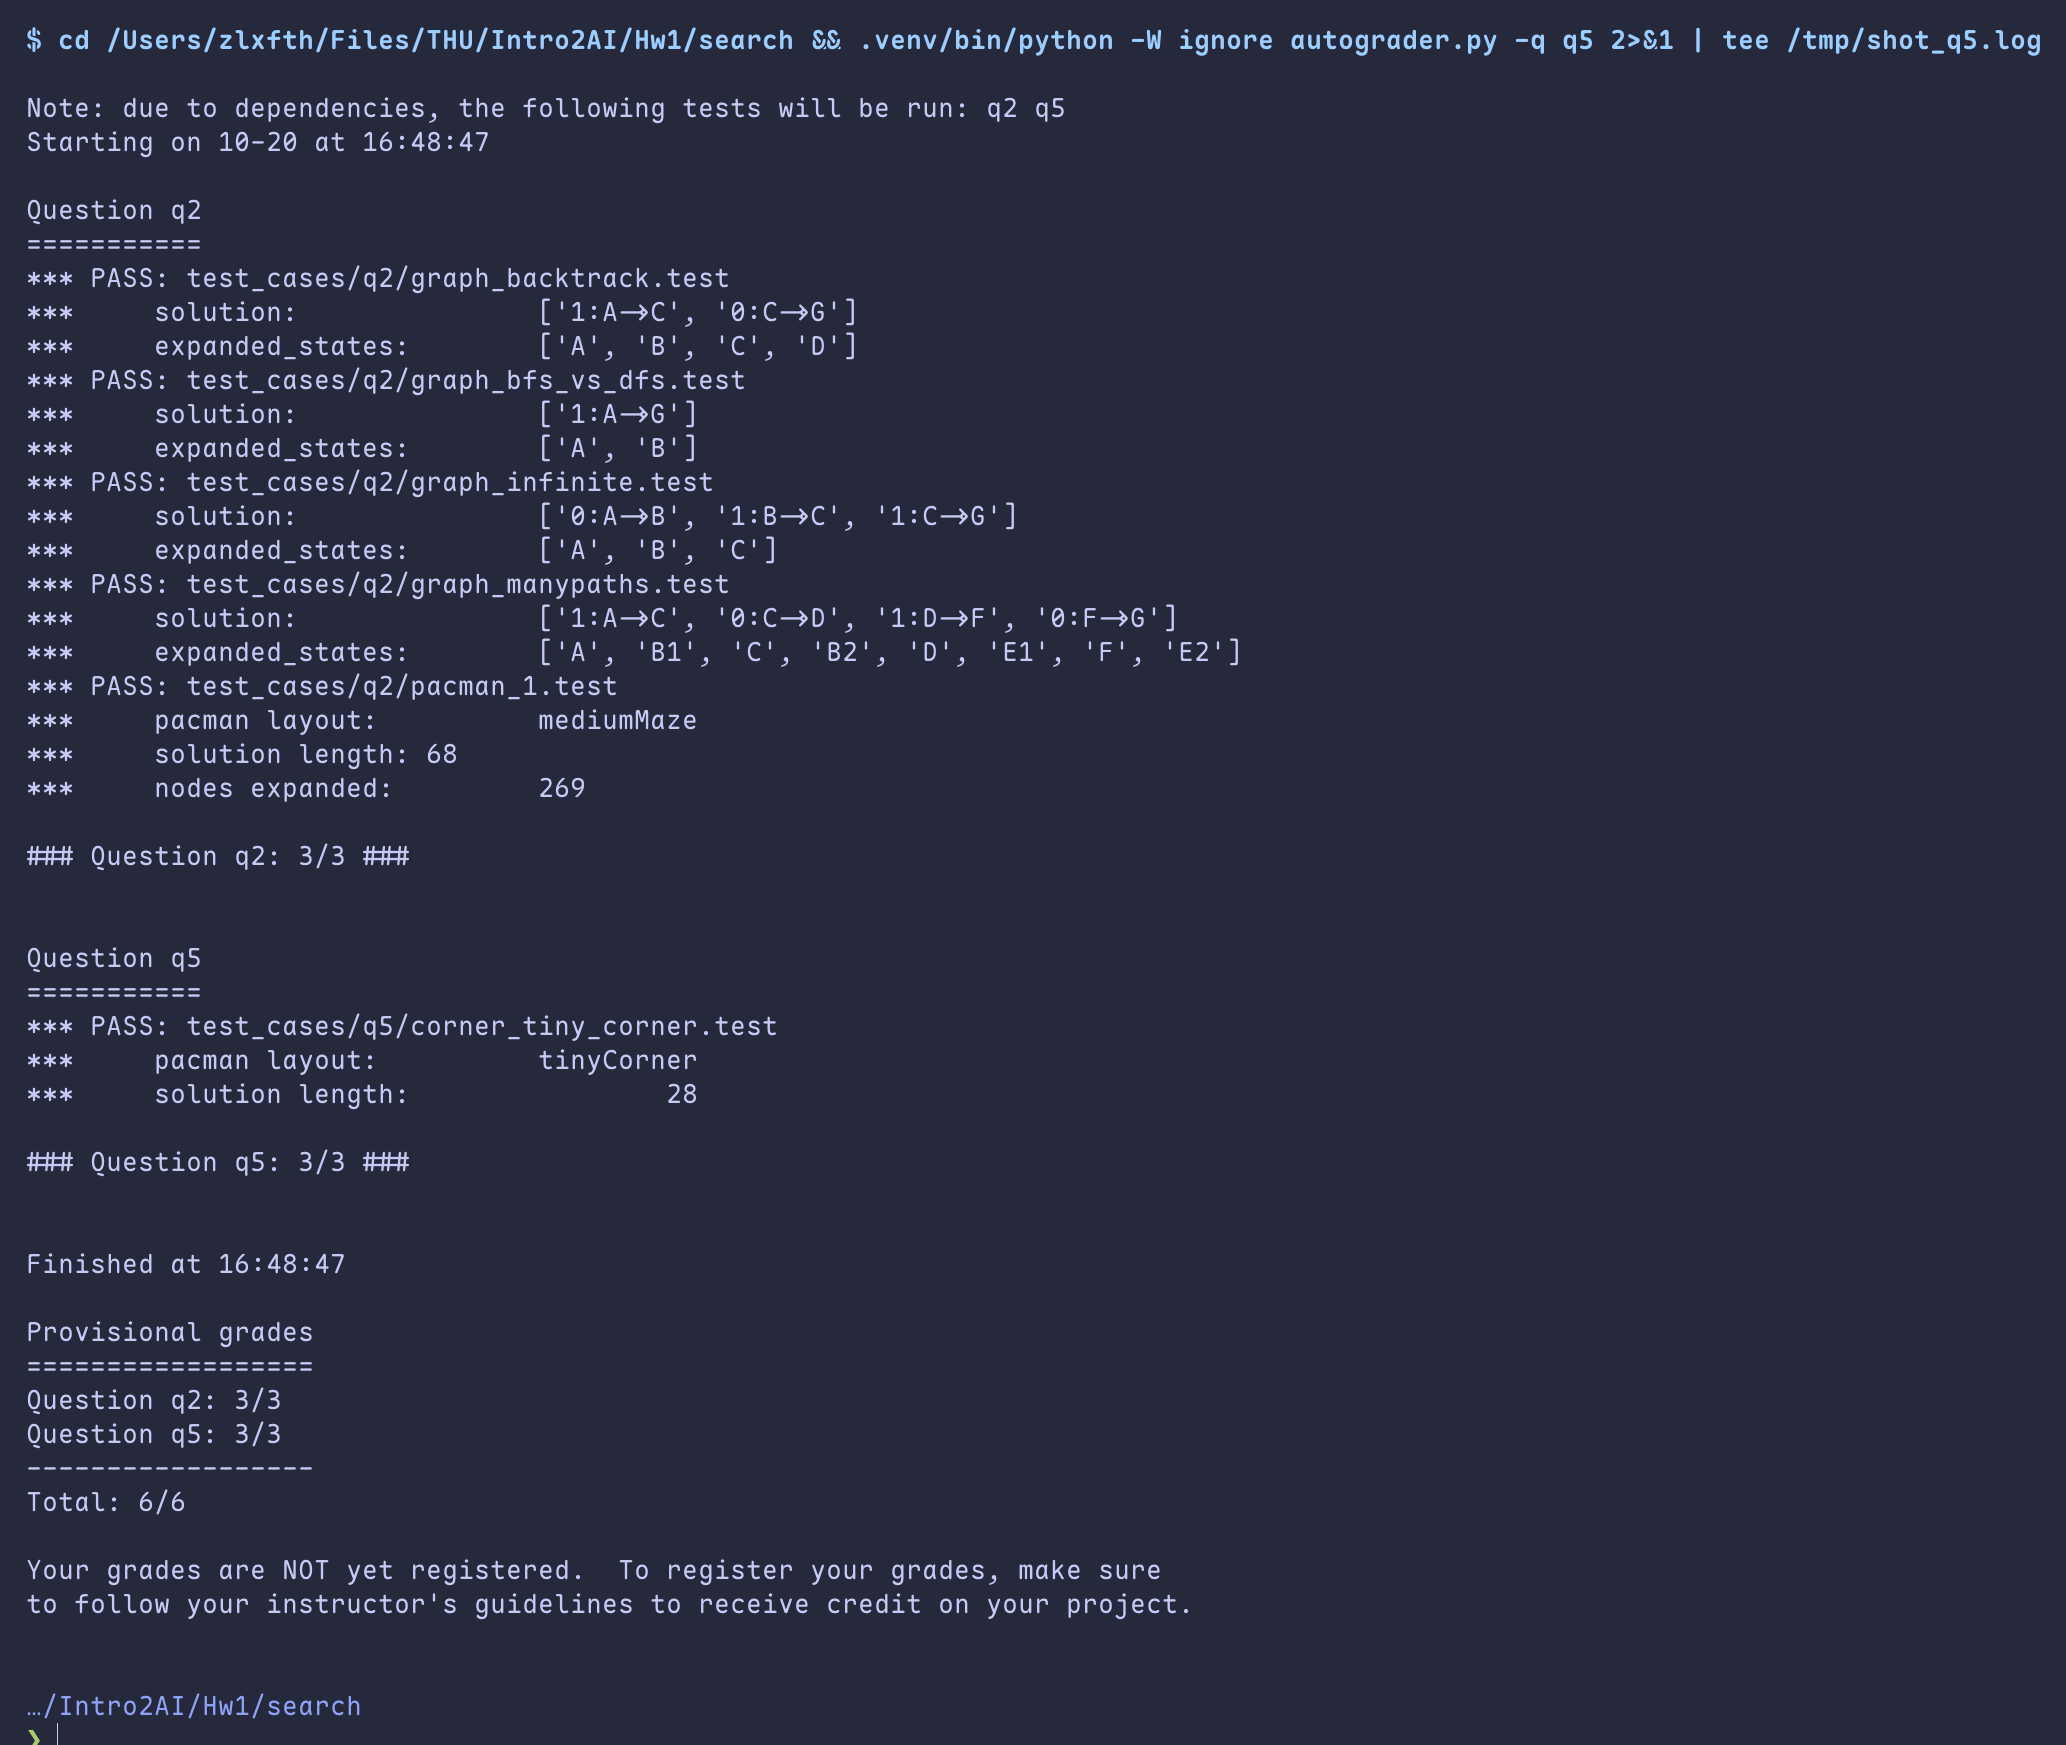
\includegraphics[width=0.78\linewidth]{../screenshot/q5.png}
\end{center}

\needspace{0.68\textheight}
\subsection*{Q2.6 Corners heuristic}
$h$ is the largest Manhattan distance to a corner not yet visited. It is
admissible (every remaining corner must be reached, so the farthest one costs at
least that much) and consistent (a step changes each distance by at most 1, and
stepping onto a corner removes a distance that is then 0). It expands 1136 nodes
instead of 1966, a 42\% reduction, comfortably below the 1200 threshold for full
credit.

\begin{center}
    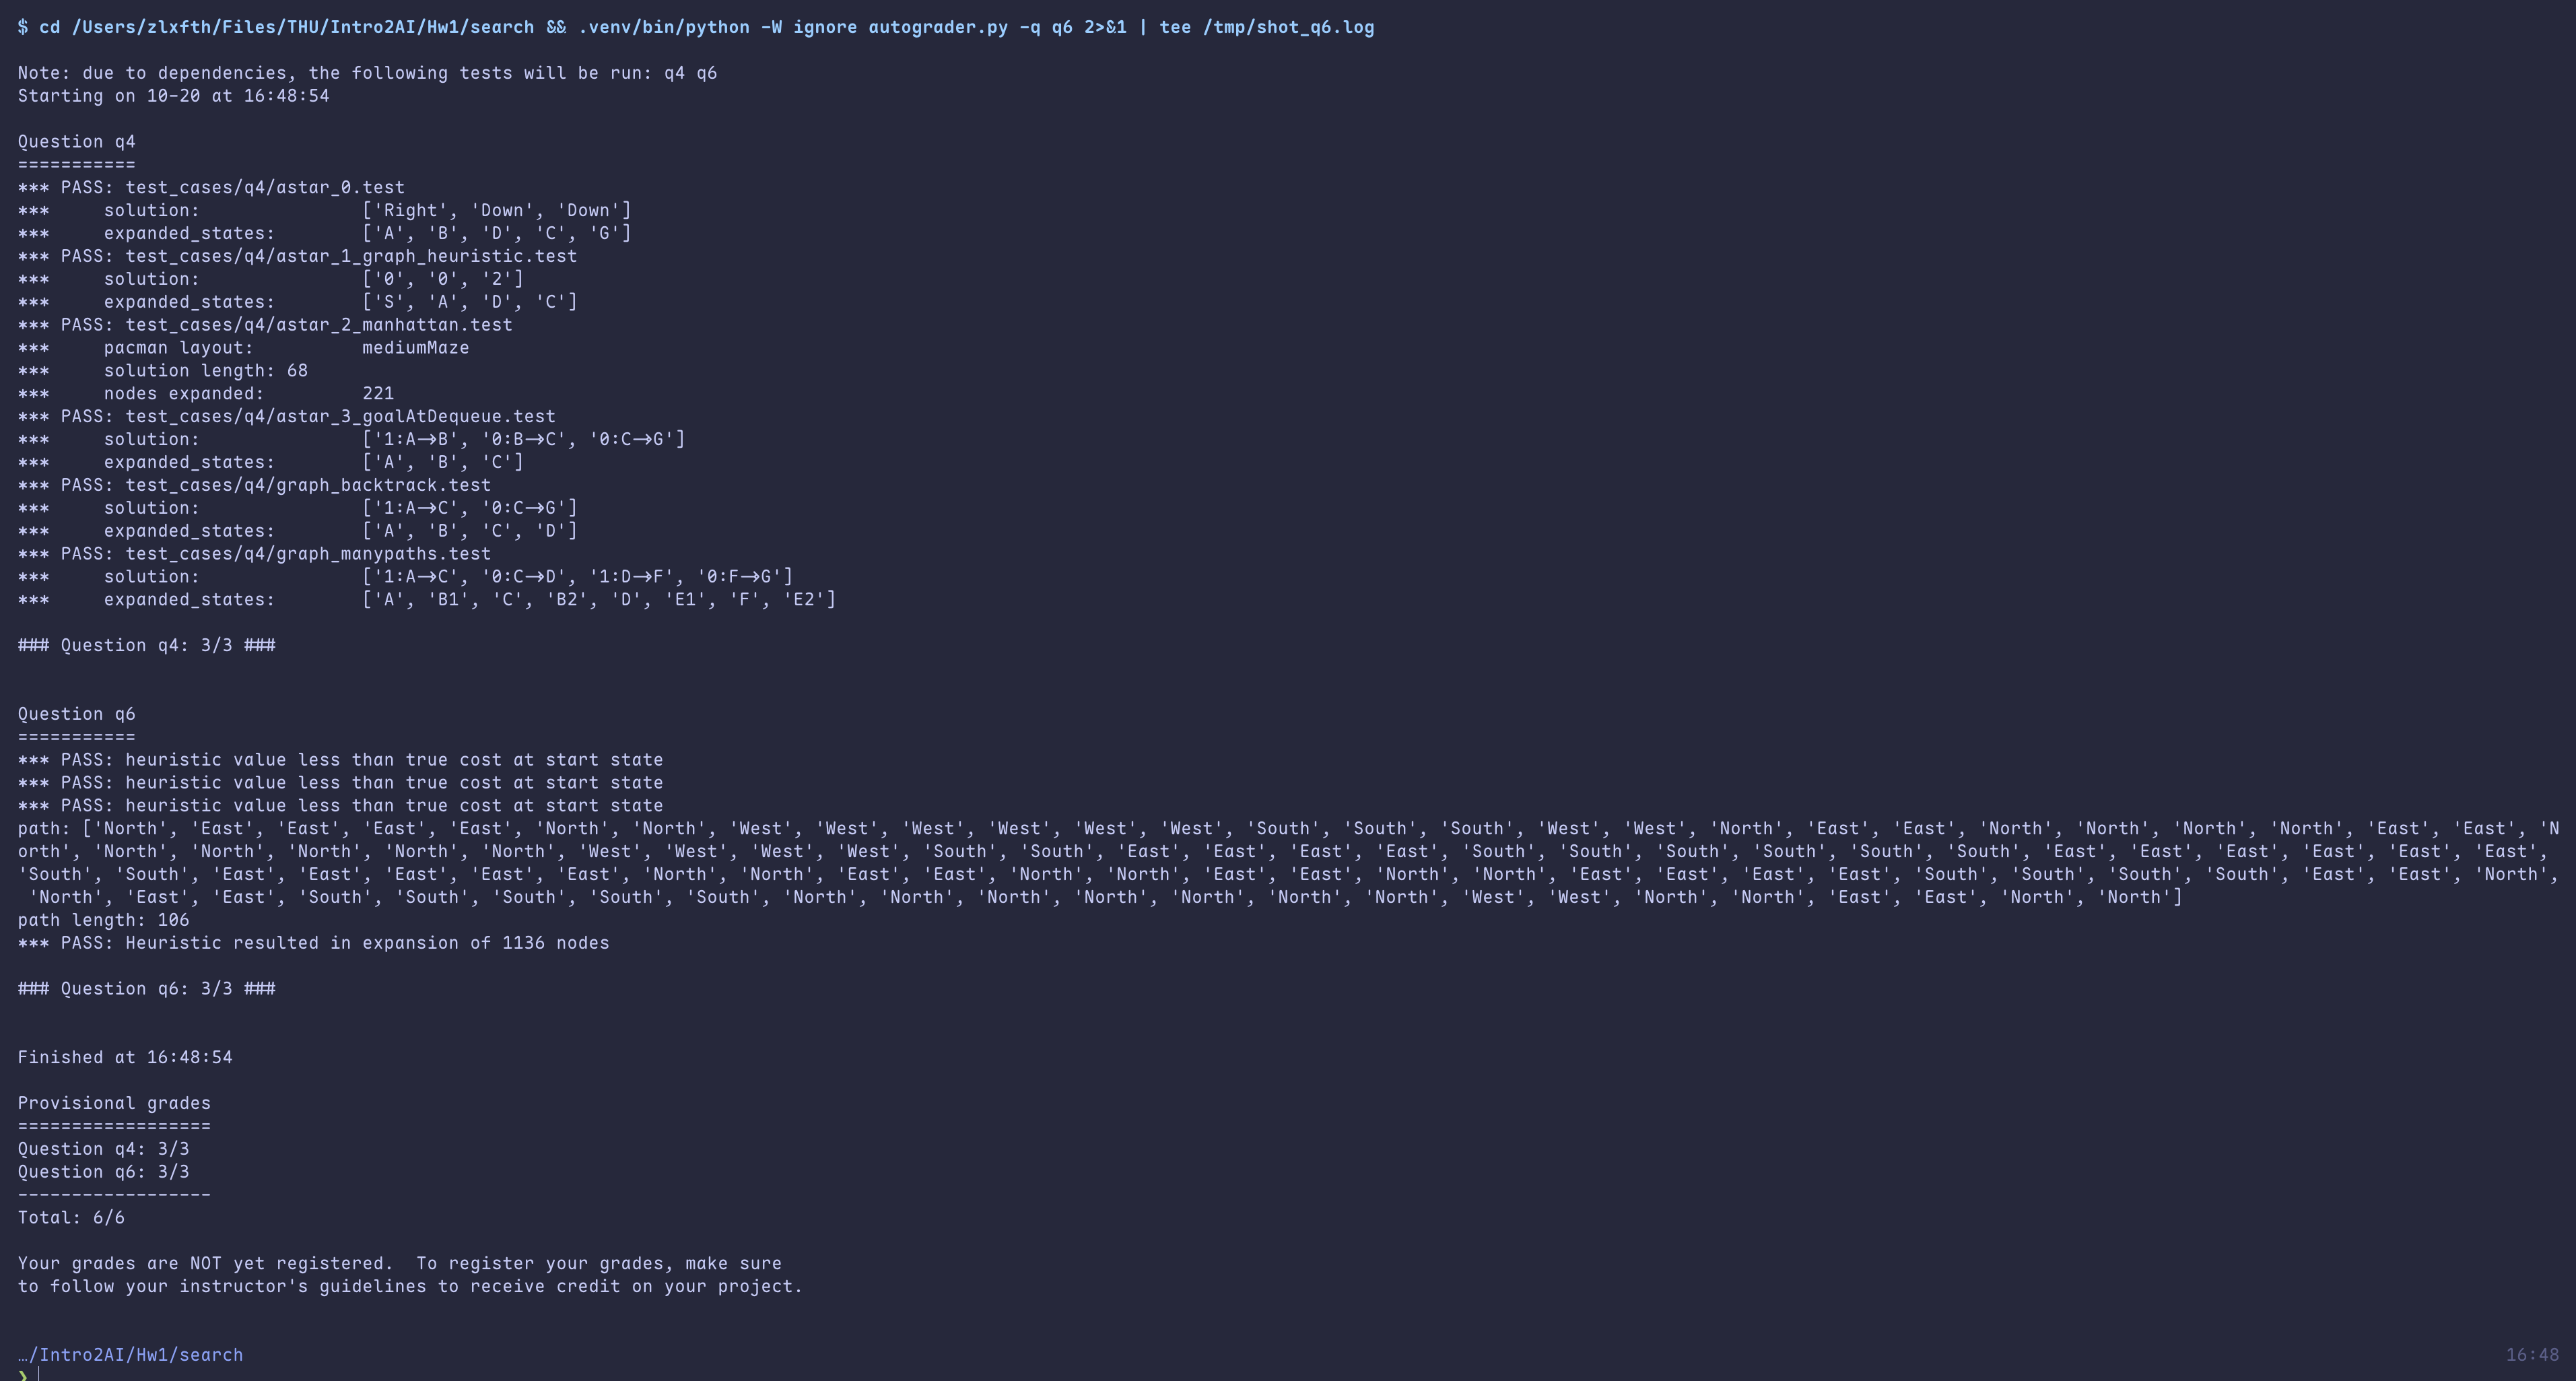
\includegraphics[width=0.92\linewidth]{../screenshot/q6.png}
\end{center}

% ===========================================================================
\clearpage
\section*{Q3}
% TODO: Programming Component 2 (Connect Four) --- Stage 1/2/3 screenshots and
%       the requested short analysis.

\end{document}
